\section{Problem Set 5}
\subsection{Control Objectives} \label{sec:control_objectives}
\subsubsection{Operational Modes}
The ultimate goal of our formation is to demonstrate on-orbit servicing of an uncontrollable target spacecraft with a swarm of one docking satellite and one observing satellite. Specifically, the Target spacecraft (SV1) has no maneuvering capabilities as it has run out of propellant, and our formation is aiming to refuel it. As such, SV1 will act as the origin of the RTN frame and remain there throughout all of our operational modes. The Watcher spacecraft (SV2) has sensing capabilities, including optical cameras such as those in the NASA Starling mission, which will be used to inspect the Target and estimate its pose for servicing purposes. The Docker spacecraft (SV3) also has optical sensors that will aid in this inspection, but also play a crucial role in proximity and docking operations. Our formation aims to demonstrate a significant advance in on-orbit pose estimation and characterization of objects, along with improved docking operations through the use of multiple spacecraft with a variety of sensor modalities. 

In order to achieve this, the significant operational modes of our formation are as follows: 

\begin{enumerate}
\item \textbf{Initial Checkout Mode} - Initial checkout of Target spacecraft with both Watcher and Docker less than a kilometer and more than 200 meters away at closest approach to allow for vision-based sensing
\item \textbf{Approach Mode} - Docker approaches the Target while Watcher watches from the same distance. This mode runs until the Docker is approximately 10 meters away from the Target
\item \textbf{Proximity Operations Mode} - Docker completes final approach Target while Watcher watches
\item \textbf{Docked Mode} - Docker docks and services Target while Watcher watches
\item \textbf{Station Keeping Mode} - Watcher and Target stay within prescribed limits of relative eccentricity and relative inclination to remain passively safe. This mode will be applied whenever the formation is not reconfiguring. 
\end{enumerate}

\subsubsection{Operational Mode ROEs}
The absolute motion of our spacecraft is not the focus, as our formation is purely concerned with servicing a satellite. As such, all of the operational modes are defined as deputy ROEs as follows. Note that the Approach mode was split into two separate waypoints (Mode 2 and Mode 3) to better illustrate the reconfiguration. 

\begin{table}[h!]
\centering
\begin{tabular}{|c|rrrrrr|rrrrrr|}
\hline
\textbf{Mode} & \multicolumn{6}{c|}{\textbf{SV2 (m)}} & \multicolumn{6}{c|}{\textbf{SV3 (m)}} \\
\cline{2-13}
 & $d_a$ & $d_\lambda$ & $d_{e_x}$ & $d_{e_y}$ & $d_{i_x}$ & $d_{i_y}$ 
 & $d_a$ & $d_\lambda$ & $d_{e_x}$ & $d_{e_y}$ & $d_{i_x}$ & $d_{i_y}$ \\
\hline
1 & 0 & 0 & 0 & 300 & 0 & 300 & 0 & 0 & 0 & 250 & 0 & -250 \\
2 & 0 & 0 & 0 & 300 & 0 & 300 & 0 & 0 & 0 & 100 & 0 & -100 \\
3 & 0 & 0 & 0 & 300 & 0 & 300 & 0 & 0 & 0 & 10  & 0 & -10 \\
4 & 0 & 0 & 0 & 300 & 0 & 300 & 0 & 0 & 0 & 1   & 0 & -1 \\
\hline
\end{tabular}
\caption{Relative Orbital Element Modes for SV2 and SV3 (scaled by $a_c$)}
\label{tab:roe_modes}
\end{table}

These ROE values were chosen to meet the minimum separation requirements outlined above, by using the following equation:

\begin{align}
R_{\min} &= \frac{\sqrt{2} \cdot a \cdot |\delta e \cdot \delta i|}%
{\sqrt{(\delta e)^2 + (\delta i)^2 + |\delta e + \delta i| \cdot |\delta e - \delta i|}}
\end{align} \label{eqn:roe_spacing}

Plotting this equation in 3D shows that the minimum distance is dominated by the minimum of the given $\delta e$ and $\delta i$, as shown by Figure \ref{fig:min_dist_contour}.
\begin{figure}[H]
    \centering
    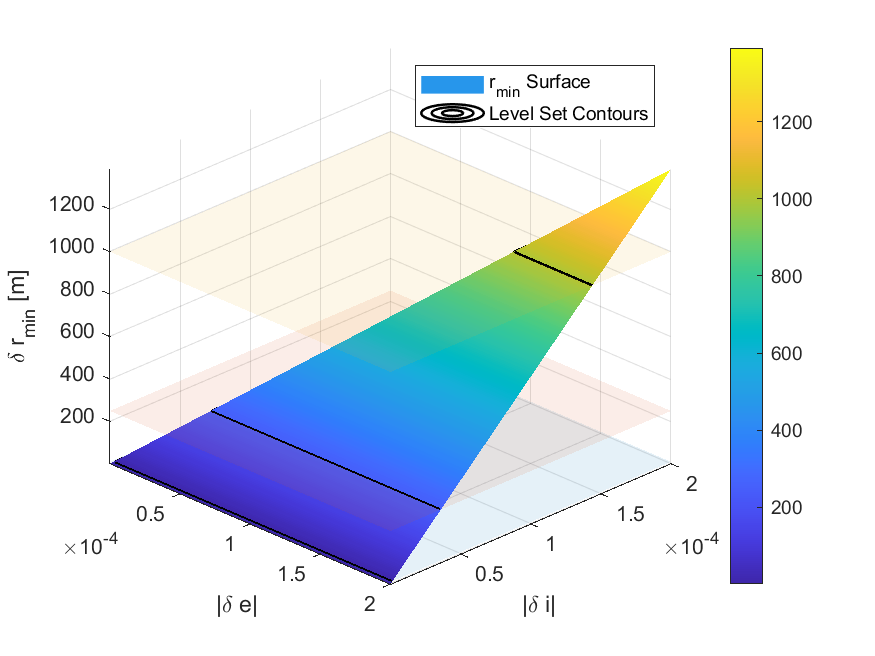
\includegraphics[width=0.75\linewidth]{sim/figures/PS5/min_dist_contour.png}
    \caption{Minimum distance contour over relative eccentricity and relative inclination}
    \label{fig:min_dist_contour}
\end{figure}
As such, $\delta e$ and $\delta i$ were chosen to be equal in magnitude for both SV2 and SV3 in order to give circular relative motion, which is helpful for maintaining the same distance throughout an orbit for the vision-based sensing on both spacecraft. Additionally, $\delta e$ and $\delta i$ were chosen to be antiparallel for SV3 (Docker) and parallel for SV2 (Watcher) to ensure that the Docker never blocks the Watcher's view of the Target by tilting the Docker's relative orbit perpendicular to the Watcher's.

\subsubsection{Formation Keeping Control Requirements}
For each station keeping mode, a keep-in region was defined for the relative eccentricity and relative inclination in order to ensure passive safety and maintain the allowable separations defined earlier. Due to the small size of the relative eccentricity and relative inclination vectors during our operational modes, a tight keep-in region of a circle with a 1-meter radius was used. 

This tight keep-in region dictates a tight relative position knowledge requirement: the Watcher's knowledge should be less than a meter and the Docker's should be less than a centimeter in order to allow for successful docking and servicing. Similarly, the velocity estimation of the Docker should be on order of mm/s.

Additionally, the actuation needed will be low-thrust, high-preicison with a low impulse bit on the order of mm/s, such as a cold gas thruster (rather than a very low-thrust option such as a Hall-effect thruster). Short, impulsive bursts will be used so to not disturb the attitude of the Docker and allow for precise control. 


\subsubsection{Reconfiguration Control Requirements}
For reconfiguration, there must always be passive safety, which is achieved through aligning the relative eccentricity and relative inclination vectors. Additionally the time to reconfigure, given in number of orbits, is prescribed for each mode below. These numbers were chosen to best illustrate the control behavior. In practice, the Approach Mode would take the longest time, especially in proximity operations where the maneuvers are small and need to be precise. 

\begin{table}[h!]
\centering
\begin{tabular}{|c|c|}
\hline
\textbf{Phase} & \textbf{Number of Orbits} \\
\hline
Station-Keeping Mode 1 & 4 \\
Mode 2 & 5 \\
Station-Keeping 2 & 4 \\
Mode 3 & 5 \\
Station-Keeping 3 & 4 \\
Mode 4 & 4 \\
\hline
\end{tabular}
\caption{Number of orbits spent in each mode and station-keeping phase} \label{tab:mode_durations}
\end{table}

\subsubsection{Choice of Actuators}
Two different types of actuators will be used. The first will be higher-thrust and lower specific impulse chemical propulsion for large maneuvers and formation reconfiguration. Electric propulsion is also an option here as it has higher specific impulse, but its low thrust makes it a poor choice for impulsive control. Another kind of actuator used with be lower-thrust propulsion, such as cold-gas thrusters. These will be used for proximity and docking operations, as fine and accurate thrust control with small impulse bits is required. 

\subsubsection{Absolute and Relative Orbit Dynamics Models}
Two dynamics models are needed: the first will be the ground-truth and the second will actually run onboard the computationally-limited spacecraft. The absolute ground-truth will be given by numerical integration of the Fundamental Orbital Differential Equation (FODE) with J2 effects for the chief and both deputies. The relative ground-truth will be calculated by taking the differences in the absolute states and converting to the RTN and ROE representations. The onboard dynamics model cannot perform numerical integration as this would be too computationally-expensive. Instead, the absolute and onboard dynamics will be given by the analytical STM with J2 for ROE as outlined in Section \ref{sec:j2_analytical_roe}, which still needs to provide accuracy as it will be used for control. 

Implementing the ground-truth model in open-loop shows each desired mode in the RTN planes as shown in Figures \ref{fig:mode_1_rtn}, \ref{fig:mode_2_rtn}, \ref{fig:mode_3_rtn}. Note that Mode 4 is not shown because SV3 does not appear in the plots due to its ROE all being 0. This ground-truth model exhibits expected J2 perturbations with a drifting relative perigee. Also note how the inclinations of the relative orbits are offset in the NT projection due to the design choice of antiparallel relative eccentricity and relative inclination vectors of SV3. All of these modes exhibit passive safety as well. 

% --- Mode 1 ---
\begin{figure}[H]
    \centering
    \begin{subfigure}[b]{0.32\linewidth}
        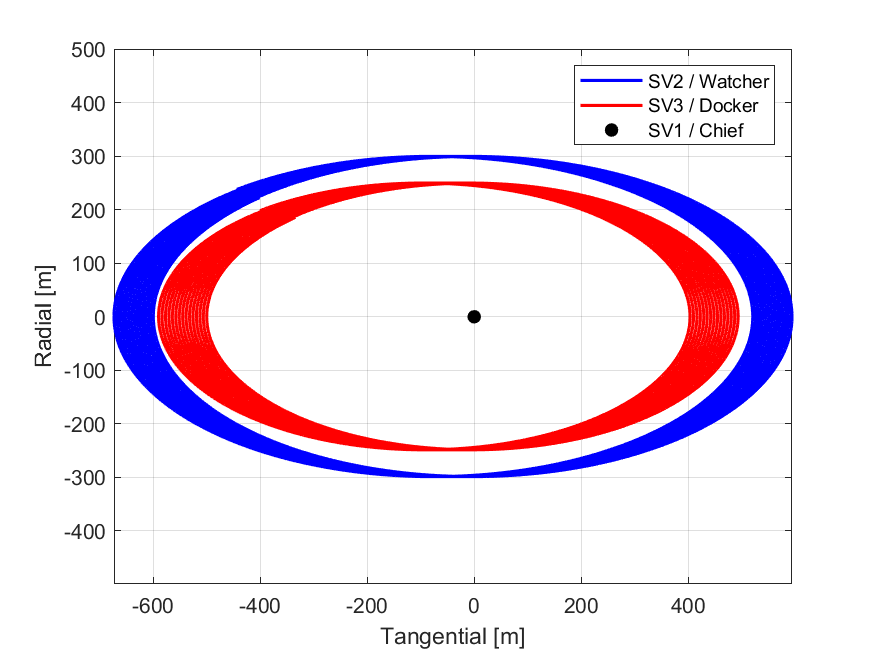
\includegraphics[width=\linewidth]{sim/figures/PS5/mode_1_RTN.png_RT.png}
        \caption{RT Projection}
        \label{fig:mode_1_rt}
    \end{subfigure}
    \begin{subfigure}[b]{0.32\linewidth}
        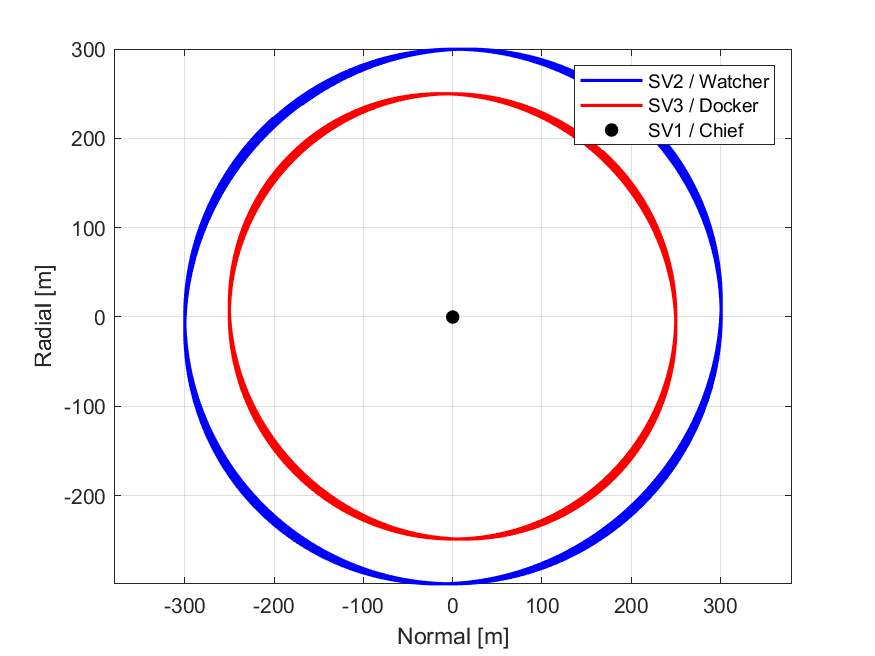
\includegraphics[width=\linewidth]{sim/figures/PS5/mode_1_RTN.png_RN.png}
        \caption{RN Projection}
        \label{fig:mode_1_rn}
    \end{subfigure}
    \begin{subfigure}[b]{0.32\linewidth}
        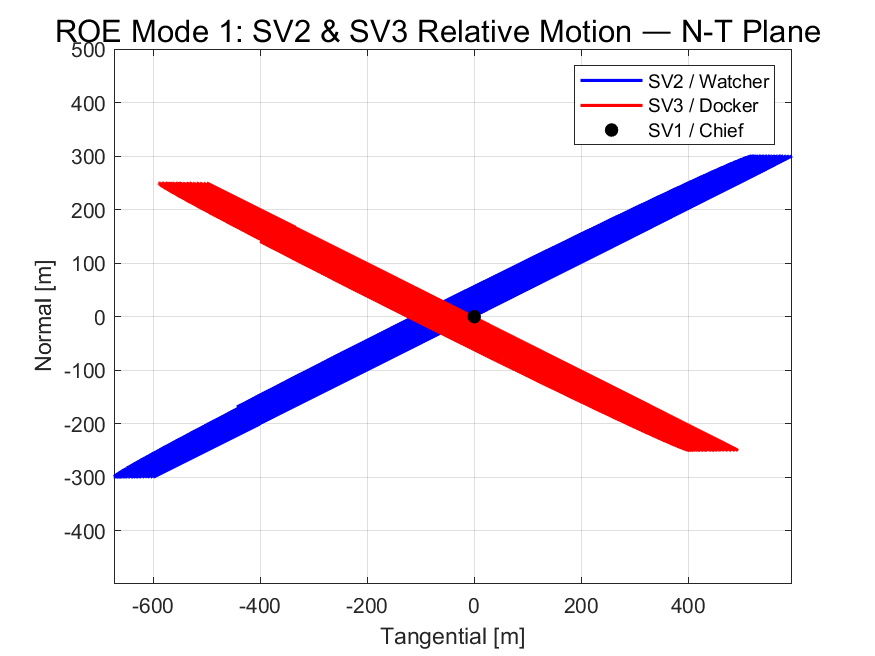
\includegraphics[width=\linewidth]{sim/figures/PS5/mode_1_RTN.png_NT.png}
        \caption{NT Projection}
        \label{fig:mode_1_nt}
    \end{subfigure}
    \caption{Mode 1 RTN Projections}
    \label{fig:mode_1_rtn}
\end{figure}

% --- Mode 2 ---
\begin{figure}[H]
    \centering
    \begin{subfigure}[b]{0.32\linewidth}
        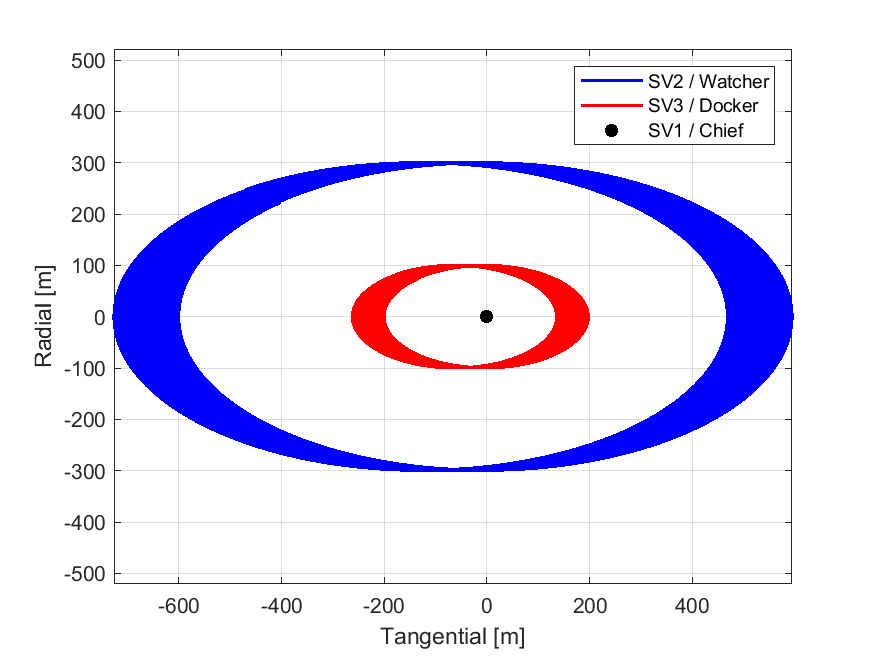
\includegraphics[width=\linewidth]{sim/figures/PS5/mode_2_RTN.png_RT.png}
        \caption{RT Projection}
        \label{fig:mode_2_rt}
    \end{subfigure}
    \begin{subfigure}[b]{0.32\linewidth}
        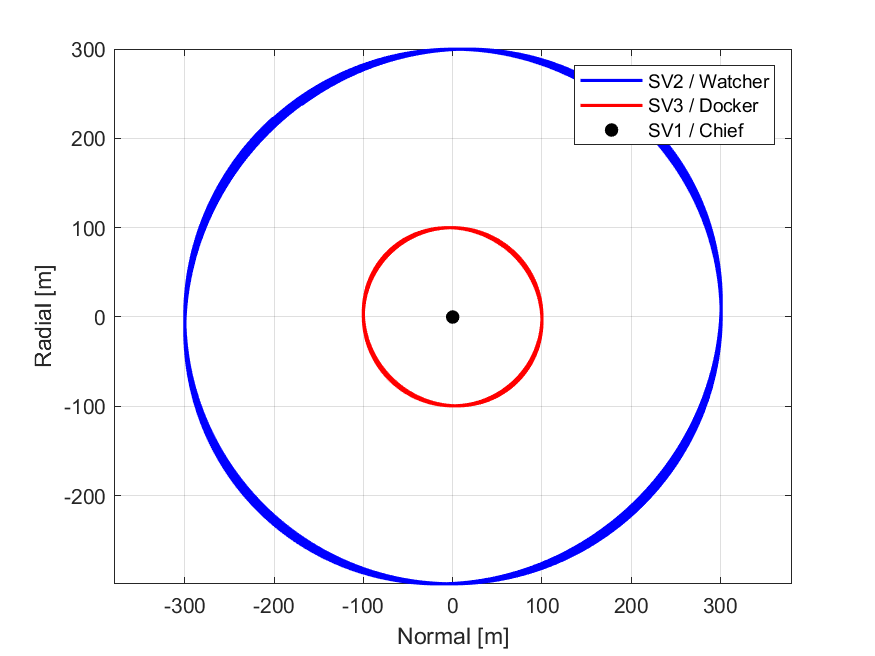
\includegraphics[width=\linewidth]{sim/figures/PS5/mode_2_RTN.png_RN.png}
        \caption{RN Projection}
        \label{fig:mode_2_rn}
    \end{subfigure}
    \begin{subfigure}[b]{0.32\linewidth}
        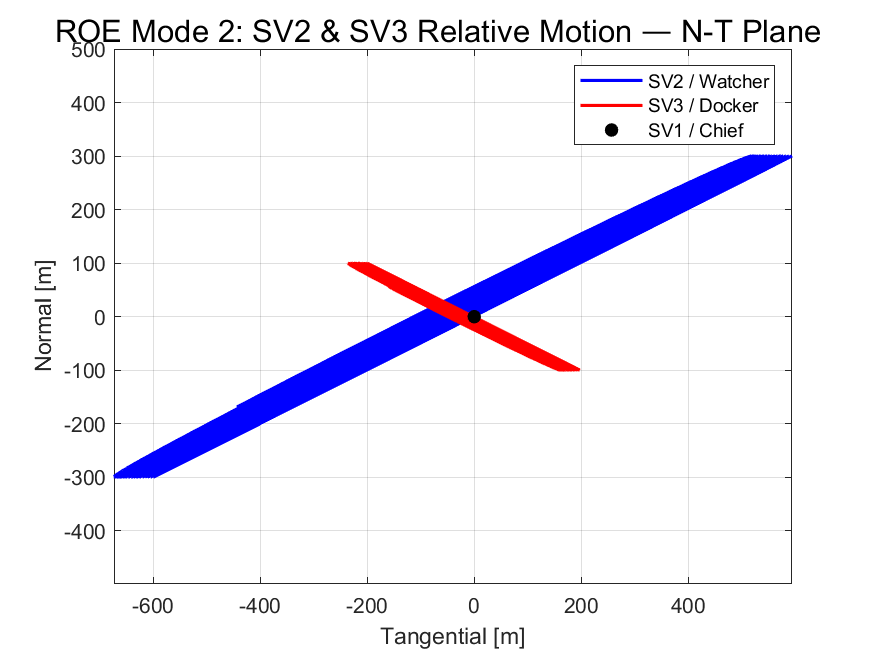
\includegraphics[width=\linewidth]{sim/figures/PS5/mode_2_RTN.png_NT.png}
        \caption{NT Projection}
        \label{fig:mode_2_nt}
    \end{subfigure}
    \caption{Mode 2 RTN Projections}
    \label{fig:mode_2_rtn}
\end{figure}

% --- Mode 3 ---
\begin{figure}[H]
    \centering
    \begin{subfigure}[b]{0.32\linewidth}
        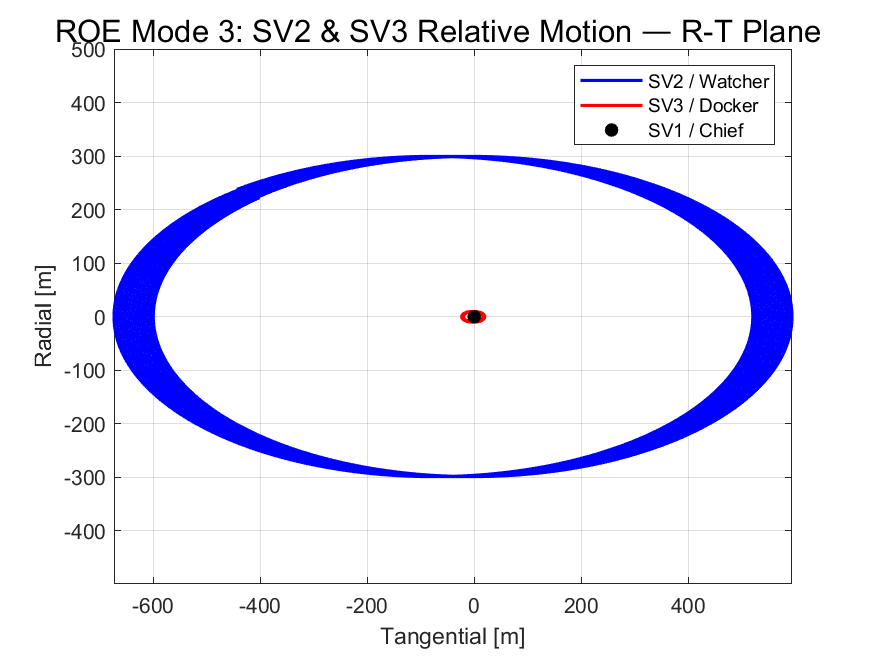
\includegraphics[width=\linewidth]{sim/figures/PS5/mode_3_RTN.png_RT.png}
        \caption{RT Projection}
        \label{fig:mode_3_rt}
    \end{subfigure}
    \begin{subfigure}[b]{0.32\linewidth}
        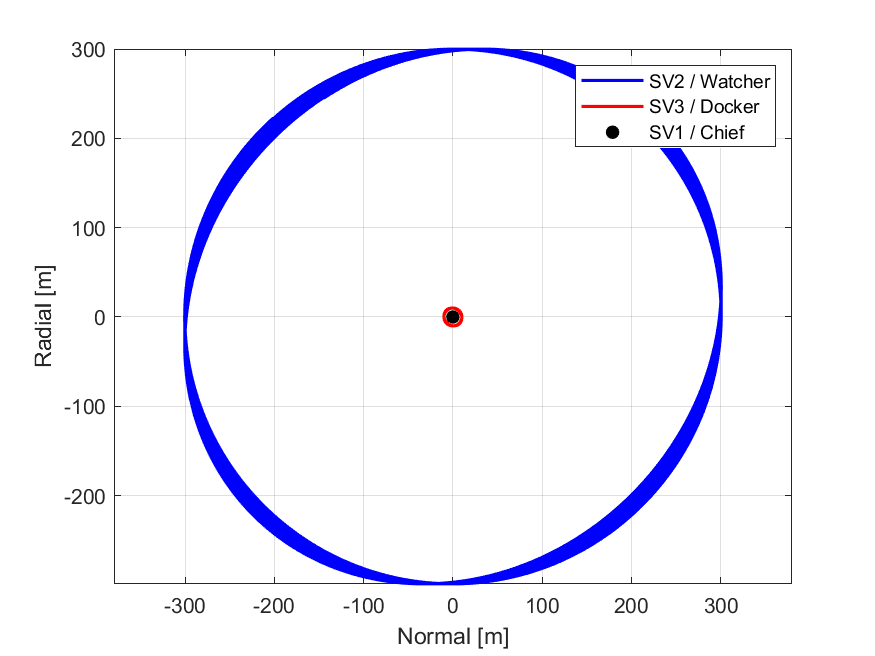
\includegraphics[width=\linewidth]{sim/figures/PS5/mode_3_RTN.png_RN.png}
        \caption{RN Projection}
        \label{fig:mode_3_rn}
    \end{subfigure}
    \begin{subfigure}[b]{0.32\linewidth}
        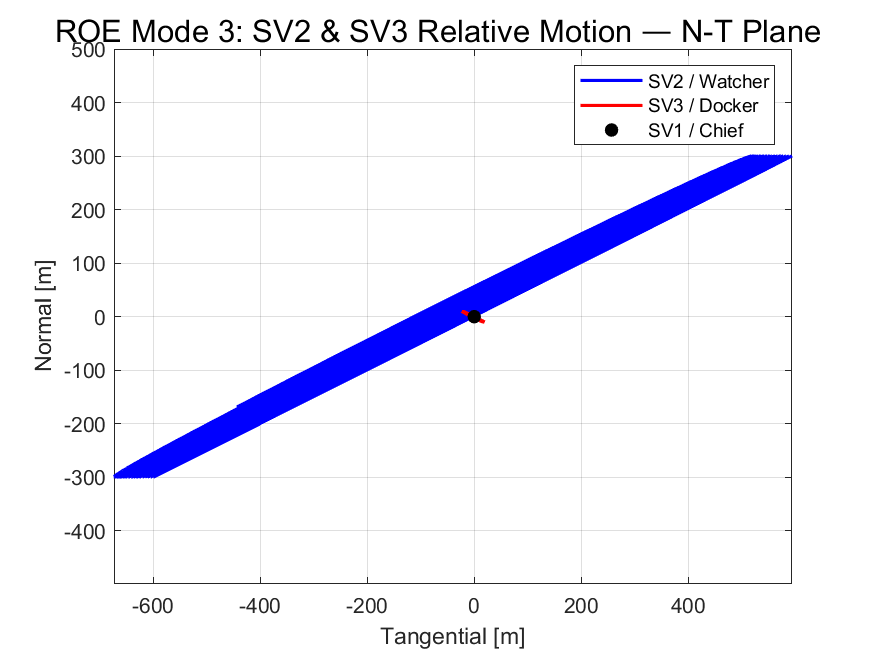
\includegraphics[width=\linewidth]{sim/figures/PS5/mode_3_RTN.png_NT.png}
        \caption{NT Projection}
        \label{fig:mode_3_nt}
    \end{subfigure}
    \caption{Mode 3 RTN Projections}
    \label{fig:mode_3_rtn}
\end{figure}

To verify that the STM is an acceptable model, it is compared in the ROE representation. As seen in Figures \ref{fig:roe_plane_compare_method} and \ref{fig:roe_time_compare_method} the STM aligns closely with the ground-truth Differences in FODE (Dif. FODE) method. The one notable exception is in the $\delta i_y$ case, although the error is very minimal.

\begin{figure}[H]
    \centering
    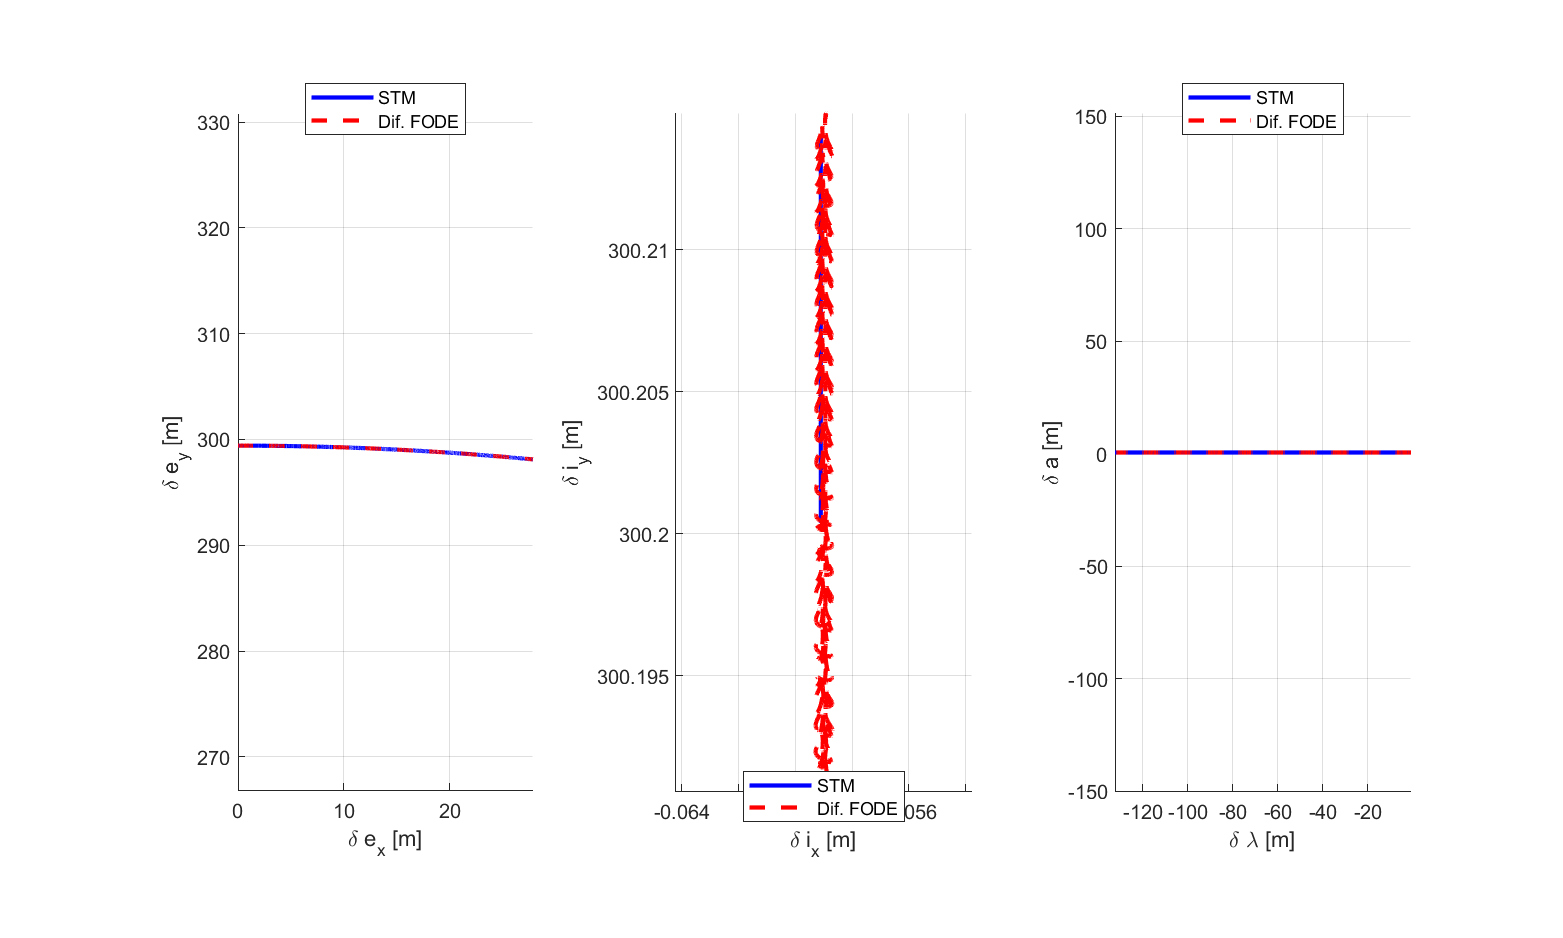
\includegraphics[width=0.75\linewidth]{sim/figures/PS5/mode_1_ROE_Planes.png}
    \caption{STM and Dif. FODE methods plotted in ROE planes}
    \label{fig:roe_plane_compare_method}
\end{figure}
\begin{figure}[H]
    \centering
    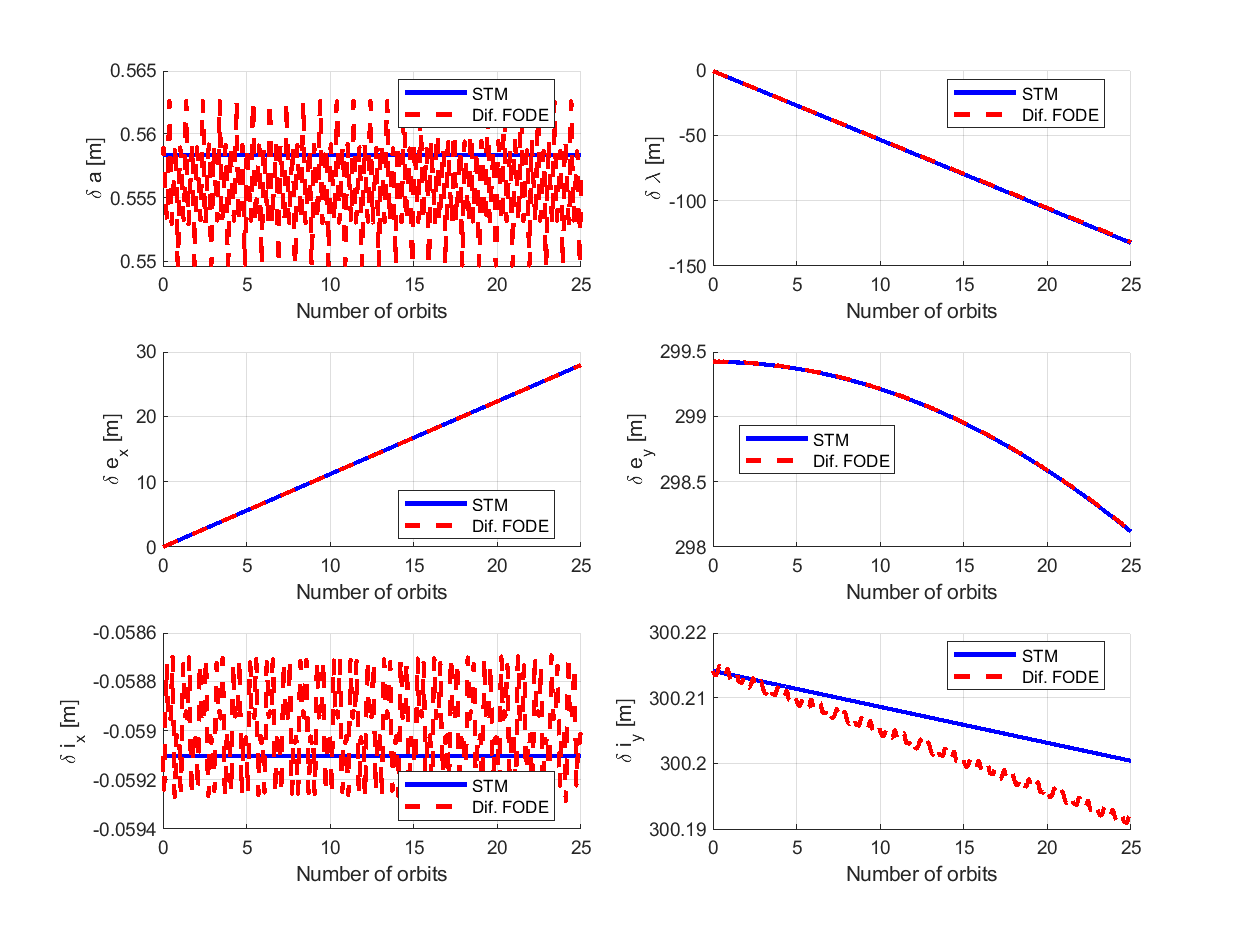
\includegraphics[width=0.75\linewidth]{sim/figures/PS5/mode_1_ROE_Time.png}
    \caption{STM and Dif. FODE methods plotted in ROE time history}
    \label{fig:roe_time_compare_method}
\end{figure}
\subsection{Impulsive Control Law}

\subsubsection{Control Method Considerations}\label{sec:control_considerations}

As highlighted in Section \ref{sec:control_objectives}, our system has four distinct operational modes, each with their own unique control accuracy and safety requirements. We also have control considerations for the maneuvers for transitioning between different modes.

Based on the requirements detailed in the previous section, we decided on the operational methods highlighted in Table \ref{tab:mode_control_methods}. Note here, that just the Docker (SV3) that performs the approach towards SV1, and so its control schemes change with time. SV2, on the other hand, keeps its original station through all modes, and does not perform any larger maneuvers (attitude maneuvers are not considered in this formulation). It only performs station-keeping corrections, if any.

\definecolor{lightgray}{gray}{0.9}

\begin{table}[H]
    \centering
    \caption{Control Methods by Mode of Operation}
    \renewcommand{\arraystretch}{1.3}

    \begin{tabularx}{\textwidth}{|>{\raggedright\arraybackslash}p{0.13\textwidth}|%
                                      >{\raggedright\arraybackslash}p{0.13\textwidth}|%
                                      >{\raggedright\arraybackslash}p{0.12\textwidth}|%
                                      >{\raggedright\arraybackslash}p{0.12\textwidth}|%
                                      >{\raggedright\arraybackslash}p{0.12\textwidth}|%
                                      >{\raggedright\arraybackslash}X|}
        \rowcolor{lightgray}
        \hline
        \textbf{Mode of Operation} & \textbf{Tracked State} & \textbf{In-plane Control Method} & \textbf{Out-of-plane Control Method} & \textbf{Control Window} & \textbf{Reasoning} \\
        \hline
        General Station Keeping (SV2 always and SV3 Mode 1) & Relative orbital elements that provide passive safety & Triplets of along-track burns & Single impulse cross-track burn & Full duration of station-keeping (see Table \ref{tab:mode_durations}) & Simple efficient control methodology that does not require prior time allocation, prevents along-track drift. \\
        \hline
        Approach Transfer (SV3 Mode 2) & Desired Mode 2 final ROE & Triplets of along-track burns & Single impulse cross-track burn & Two orbits for transfer & Simple efficient control methodology that does not require prior time allocation, prevents along-track drift. \\
        \hline
        Proximity Maneuvers (SV3 Mode 3) & Desired Mode 3 final ROE & Radial impulse burns & Single-impulse cross-track burn & Two orbits for transfer & Provides tight control, no plume on target satellite. \\
        \hline
        Docked Station Keeping (SV3 Mode 4) & N/A (Docked State) & No in-plane control & No out-of-plane control & Service duration & Rigid-body docking eliminates relative motion; no active control required. \\
        \hline
    \end{tabularx}
    \label{tab:mode_control_methods}
\end{table}



\subsubsection{Control Maneuver Formulations}

% Although we had the different ideas for control methodologies for the different modes, during the duration of this submission we were only able to get one method working exactly to meet our requirements: naive least squares. 
Multiple techniques for control were implemented for both in-plane and out-of-plane control: closed-form solutions for ROE control in perturbed near-circular orbits provided in \cite{chernick2018new}, and a naive least squares method for control of all ROEs simultaneously. 
% However, the method from \cite{damicothesis} causes a drift in the $\delta \lambda$ that we were not able to close (likely with a third burn). We were also unable to complete a working implementation of the closed-form solution. Although these will be discussed in later submissions (to cover all the methods detailed in Table \ref{tab:mode_control_methods}), here we will primarily discuss the naive-least squares method. 
These methods are discussed below. In the original PSET 5 submission, the Naive least squares method was the primary mode of control. During the final submission, other methods were implemented for significantly improved impulsive-control performance.

\textit{\textbf{Naive Least-Squares Method}}\\
The naive least-squares method works on the principle that a sequence of relative orbital elements can be related to each other with a linearized model that accounts for J2 perturbations, called a state transition matrix. This STM was previously stated in Equations \ref{eq:stm_matrix} and \ref{eq:state_transition_relation}. 

The change in relative orbital elements $\Delta \delta \alpha$ can also be related to the applied $\Delta v$ as \cite{chernick2021optimal}
\begin{align}
    \boldsymbol{\Delta \delta \alpha} = \Gamma\Delta \boldsymbol{v}
\end{align} \label{eq:delta_v_to_alpha}
Putting these together, we have a formulation for a set of control maneuvers $\Delta v$ required to achieve a desired change in relative orbital elements.
\begin{align}
\Delta \delta \boldsymbol{\alpha} = \delta \boldsymbol{\alpha}(t_f) - \Phi_{f,0} \, \delta \boldsymbol{\alpha}(t_0)
= \sum_{k = 1}^{M} \Phi(t_k) \Gamma (t_k)  \delta \mathbf{v}_k 
\end{align} \label{eq:delta_v_to_delta_alpha}
From theoretical formulations, we adopt the standard of setting three equally-spaced in time $\Delta v$ impulses for in-plane maneuvers, or a single impulse burn $\Delta v$ for out-of-plane maneuvers.
For near-circular orbit, the transformation matrix $\Gamma$ is given simply by
\begin{align}
\Delta \delta \boldsymbol{\alpha}_k = \Gamma_k \delta \mathbf{v}_k = \frac{1}{na}
\begin{bmatrix}
0 & 2 & 0 \\
-2 & 0 & 0 \\
\sin(u_k) & 2\cos(u_k) & 0 \\
-\cos(u_k) & 2\sin(u_k) & 0 \\
0 & 0 & \cos(u_k) \\
0 & 0 & \sin(u_k)
\end{bmatrix}
\begin{bmatrix}
\delta v_R \\
\delta v_T \\
\delta v_N
\end{bmatrix}
\end{align}

where $\Delta v$ is in the RTN frame, and $a$ is the semi-major axis of the chief SV1. We can also relate the mean argument of latitude to the maneuver time using the formulation

\begin{align}
    u_k = t_{k} \left( n + \kappa \left( \eta P + Q \right) \right) + u_{0}
\end{align}

where $P, Q, \eta, \kappa$ are defined in Equation \ref{eq:stm_matrix}.

The control maneuvers are solved by applying least-squares the linear system $M\delta v = \delta a$ which is formed by stacking all the states in the summation of Equation \ref{eq:delta_v_to_delta_alpha}.

\begin{equation}
\left[
\Phi_1 \mathbf{\Gamma}_1 \quad
\Phi_2 \mathbf{\Gamma}_2 \quad
\cdots \quad
\Phi_N \mathbf{\Gamma}_N
\right]
\begin{bmatrix}
\delta \mathbf{v}_1 \\
\delta \mathbf{v}_2 \\
\vdots \\
\delta \mathbf{v}_N
\end{bmatrix}
= M_{[6,3N]} \delta \mathbf{v}_{[3N,1]} = \Delta \delta \boldsymbol{\alpha}
\end{equation}

Using a pseudo-inverse for an analytical least-squares solution 

\begin{align}
    \delta \mathbf{v} = M^\top (M M^\top)^{-1} \Delta \delta \boldsymbol{\alpha}
\end{align}

This is our control solution, and is applied in the FODE simulation described in the following section.

\textit{\textbf{Triplet of Tangential Burns for In-Plane Control}}\\

In our relative orbit re-configurations, the primary in-plane change is in $\delta e_y$. At the end of each reconfiguration, $\delta a$ and $\delta \lambda$ are ideally zero. This is a control case with the change in eccentricity vector dominant. For this, \cite{chernick2018new} provides a three tangential burn control method that controls the in-plane ROEs. The result is derived from the variational equations that relate the tangential burns to the change in the ROEs, shown below.

\begin{align}
    2(\delta v_{T1} + \delta v_{T2} + \delta v_{T3}) &= n a \Delta \bar{a} \\
    -q \, \delta v_{T1} - p \, \delta v_{T2} - l \, \delta v_{T3} &= n a \Delta \bar{\lambda} \\
    2 \cos(U_1) \delta v_{T1} + 2 \cos(U_2) \delta v_{T2} + 2 \cos(U_3) \delta v_{T3} &= n a \Delta \delta_{e_x} \\
    2 \sin(U_1) \delta v_{T1} + 2 \sin(U_2) \delta v_{T2} + 2 \sin(U_3) \delta v_{T3} &= n a \Delta \delta_{e_y}
\end{align}

where 
\begin{align}
    q &= \left( u_f - u_{T1} - \frac{c}{1 - c} u_f \right) \\
    p &= \left( u_f - u_{T2} - \frac{c}{1 - c} u_f \right) \\
    l &= \left( u_f - u_{T3} - \frac{c}{1 - c} u_f \right) \\
    U_i &= (1 - c) u_{Ti} + c u_f \\
    c &= \frac{\dot{\omega}}{n + \kappa (\eta P + Q)}
\end{align}.

Based on this, \cite{chernick2018new} provides a formulation for $\Delta v_{T1}, \Delta v_{T2}, \Delta v_{T3}$ in Tables 3 and 4. The burns are separated by mean longitude $u$ of $k\pi$ radians, i.e. on opposite ends of the near-circular orbit. 

\textit{\textbf{Single-burn Relative Inclination Control}}\\

Relative inclination can be controlled by a single burn in the cross-track direction. This result is also provided in \cite{chernick2018new}, which provides a formulation for near-circular orbits that also accounts for J2 perturbations.


\textit{\textbf{Pair of Radial Burns for In-Plane Control}}\\

\textbf{\textit{Setup Formulation}} \\
The setup of the formation reconfigurations and what we want to solve are highlighted in Section \ref{sec:control_objectives}.

\textbf{\textit{Comparing delta-v}} \\
% The comparison of the least-squares method with the lower-bound delta-v $\Delta v_{lb}$ is provided in Table \ref{tab:dv_comparison}.
The comparison of our final control configuration $\Delta v$ with the lower-bound delta-v $\Delta v_{lb}$ is provided in Table \ref{tab:dv_comparison}.

\textbf{\textit{Station-Keeping Maneuvers}}

Station-keeping is implemented in the station-keeping periods between large maneuver modes to prevent satellite drift in an incorrect direction. Specifically, our method calls the naive-least squares formulation (as described in the previous section) to find impulsive maneuvers that bring the satellite back to the desired relative orbital elements.
\begin{figure}[H]
    \centering
    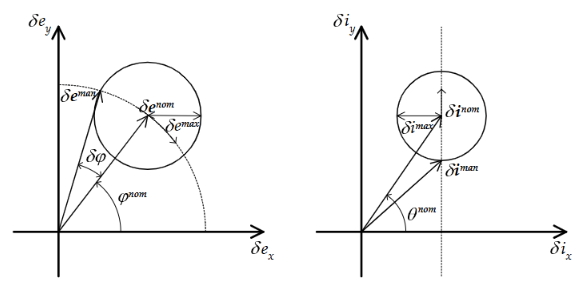
\includegraphics[width=0.75\linewidth]{sim//figures//PS5/station_keeping_man_damico.png}
    \caption{Station keeping the relative eccentricity and inclination vectors \cite{damicothesis}}
    \label{fig:station_keeping_guide}
\end{figure}

Based on Figure \ref{fig:station_keeping_guide}, we calculate the required relative orbital elements $\delta e_{man}$ and $\delta i_{man}$ that put us on the other end of the safety window. The safety window is determined by the control requirements and Equation \ref{eqn:roe_spacing}.

\subsubsection{Justificiation and Implementation of Control}

\textbf{\textit{Dynamics Model for Ground Truth Simulation}}

For our ground-truth simulation model, we utilized a FODE simulation model that is described in Section \ref{sec:fode_simulation}. This model gives us a high-fidelity model in which it is simple to incorporate J2 perturbations and drag models (although the drag models have not been implemented yet). The states of the satellites are stored and propagated in ECI co-ordinates. 

When simulating a maneuver, the propagation is stopped, the required $\delta v$ is added to the state, and then the propagation is continued. This allows us to simulate the impulsive burns. The $\delta v$ burns, which are calculated in RTN frame as a result of the naive least-squares and converted to ECI based on the chief's state at maneuver time.

% Separate from the primary simulation that implemented the different modes and maneuvers, we implemented a more integrated simulation for station-keeping that continuously plans maneuvers if the eccentricity vector or inclination vector go beyond the safe region. The code structure for station keeping, which will also simulate the primary larger maneuvers in the future, is shown in Algorithm \ref{alg:station_keeping}.

% \begin{algorithm}[H]
% \caption{Station=keeping Simulation and Plotting}
% \begin{algorithmic}[1]

% \State Initialize time array, chief semi-major axis, and empty state histories
% \State Extract nominal ROE for SV2 and SV3
% \State Define station-keeping bounds
% \State Compute desired eccentricity offsets

% \For{each time step $t_i$ in $t_{\text{series}}$}
%     \State Propagate SV1, SV2, SV3 states using RK4
%     \State Convert SV2 and SV3 states to ROE w.r.t. SV1

%     \If{SV has not yet performed control}
%         \If{eccentricity deviation exceeds threshold}
%             \State Compute station keeping maneuver with naive least squares (3 burns)
%             \State Store SV $\Delta v$ for eccentricity control
%         \EndIf
%         \If{inclination deviation exceeds threshold}
%             \State Compute station keeping maneuver with naive least squares (1 burn)
%             \State Store SV $\Delta v$ for inclination control
%         \EndIf
%     \EndIf
%     \If{a planned SV $\Delta v$ is scheduled now}
%         \State Apply $\Delta v$ to SV and remove it from queue
%     \EndIf
% \EndFor

% \State Convert SV2 and SV3 final states to RTN position relative to SV1\EndProcedure
% \end{algorithmic}
% \end{algorithm} \label{alg:station_keeping}

\textbf{\textit{Selection of Dynamics Model for Controller}} \\
The naive least-squares utilizes the STM for near-circular orbits detailed in Equation \ref{eq:stm_matrix} to propagate the state. Control maneuvers calculate $\delta v$ in the RTN frame, the input and reference ROEs use quasi-nonsingular relative orbital elements.

\textbf{\textit{Actuator Implementation, Sensor and Disturbance Models}} \\
For this submission, considerations of the delta-v budget, actuator implementation, sensor models, and disturbance models (apart from J2) are ignored. These other practical considerations will be incorporated in future submissions.

\subsubsection{Results and Analysis of Control Performance} \label{sec:analysis_of_control}

The results of the control system are shown in the following figures. These results also include the station-keeping control between modes. However, this station-keeping method behaves oddly, and does not do a satisfactory job in maintaining the current relative orbital elements.

Figures \ref{fig:roe_planes_modes} and \ref{fig:roe_time_modes} show the desired and actual ROEs for each mode. $\delta a$ becomes non-zero during the maneuvers because there are along-track elements. However, at the end of each mode, the control system is able to reduce $\delta a$ to near zero. But due to $\delta a$ and $\delta i_x$ not being precisely zero throughout the control and station-keeping modes, a drift is introduced in $\delta \lambda$. $\delta e_x$ and $\delta i_x$ are always meant to be zero, but again the maneuvers introduce variations. Each control mode tries to return $\delta e_x$ and $\delta i_x$ to zero but is unable to get all the way there. $\delta e_y$ and $\delta i_y$ exhibit the most accurate behavior. The control system is able to reach the desired $\delta e_y$ and $\delta i_y$ in each mode with very little error. This is important because these are the only non-zero factors in the desired ROEs and drive passive safety. 

\begin{figure}[H]
    \centering
    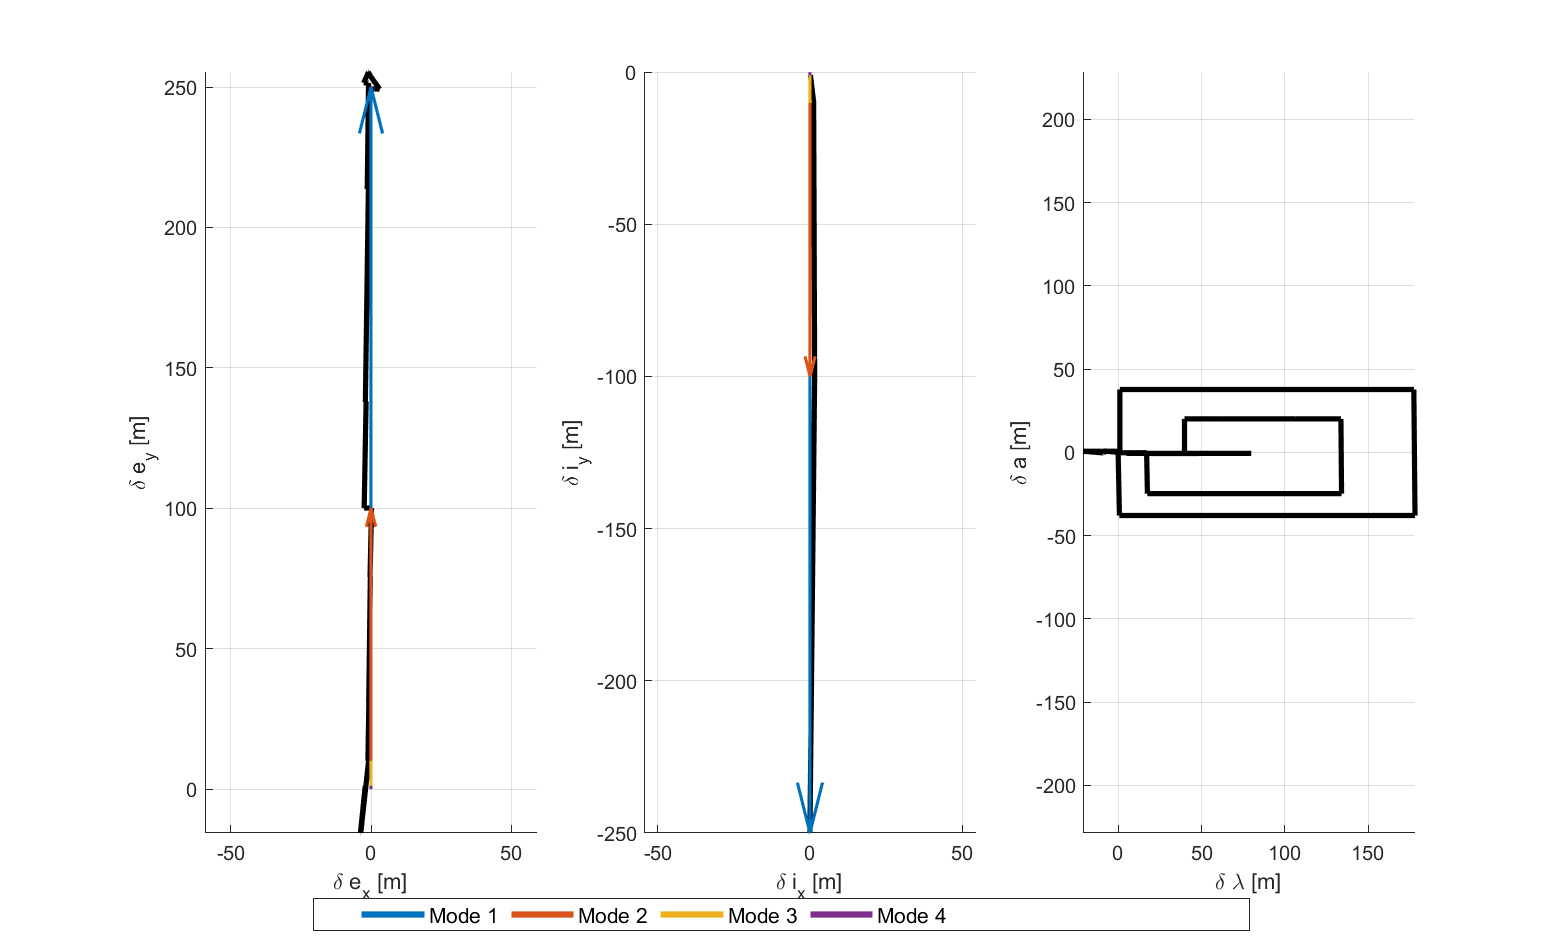
\includegraphics[width=0.75\linewidth]{sim/figures/PS5/ROE_planes_modes_SV3.png}
    \caption{Actual and desired ROE plotted for all modes in ROE planes, SV3}
    \label{fig:roe_planes_modes}
\end{figure}
\begin{figure}[H]
    \centering
    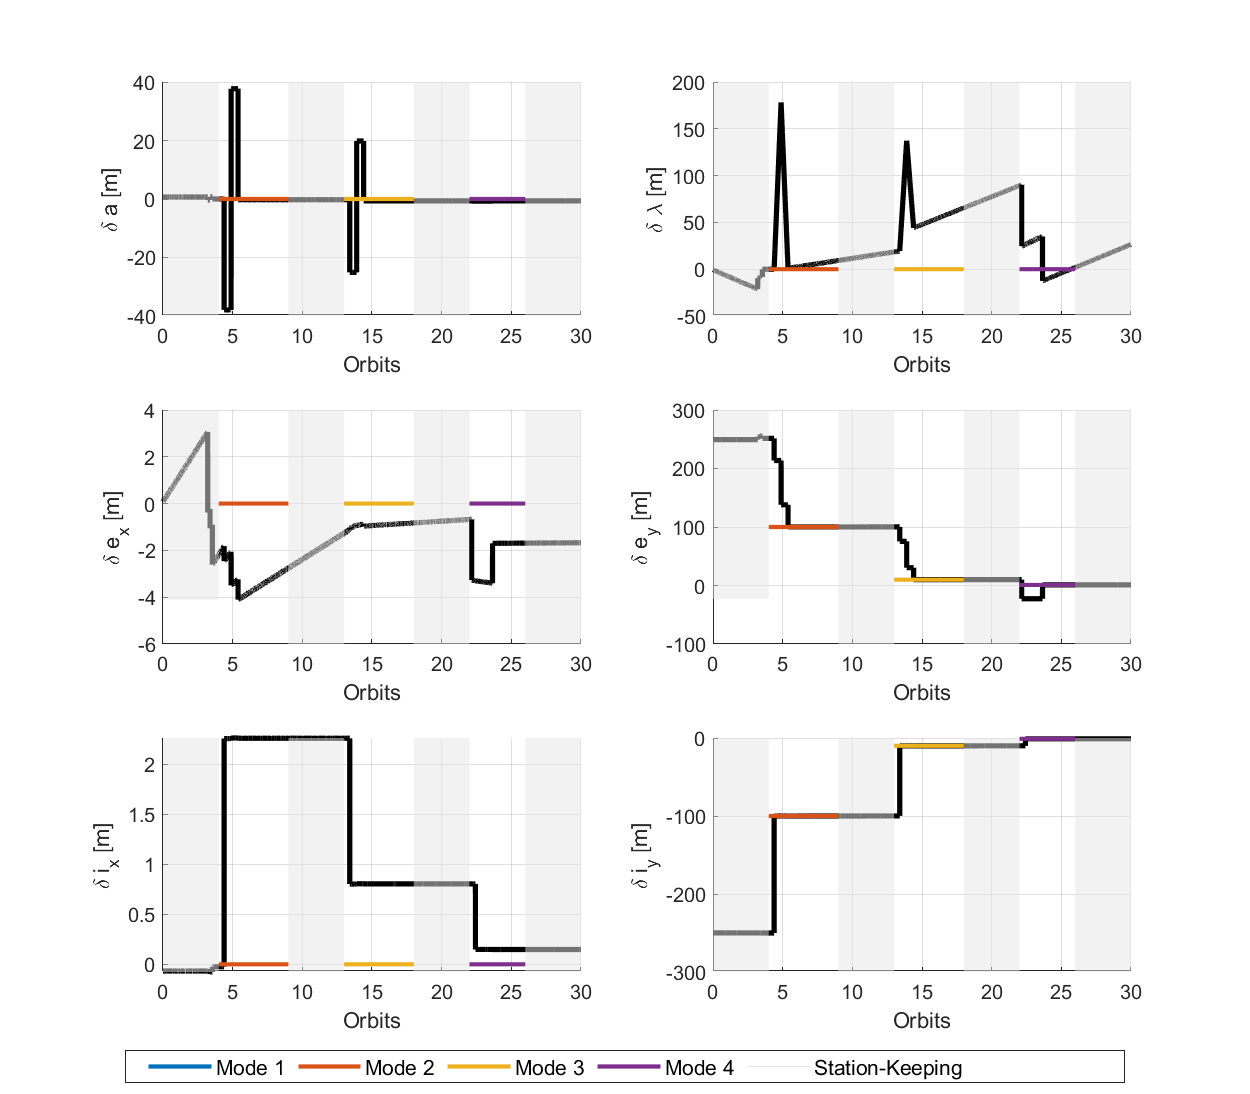
\includegraphics[width=0.75\linewidth]{sim/figures/PS5/ROE_over_time_modes_SV3.png}
    \caption{Actual and desired ROE plotted for all modes in ROE time history, SV3}
    \label{fig:roe_time_modes}
\end{figure}

Figure \ref{fig:roe_error_time_modes} reflects the same behavior in the tracking errors. The control system is able to track $\delta a, \delta e_y, and \delta i_y$ very well. The other tracking errors can be corrected either through station-keeping control or the usage of another control method. The naive least-squares method produces delta-v's that are in all directions in RTN. Other closed-form approaches, such as reachable set theory are able to specify more precise maneuvers that do not have as many unwanted side effects on other ROEs. 

\begin{figure}[H]
    \centering
    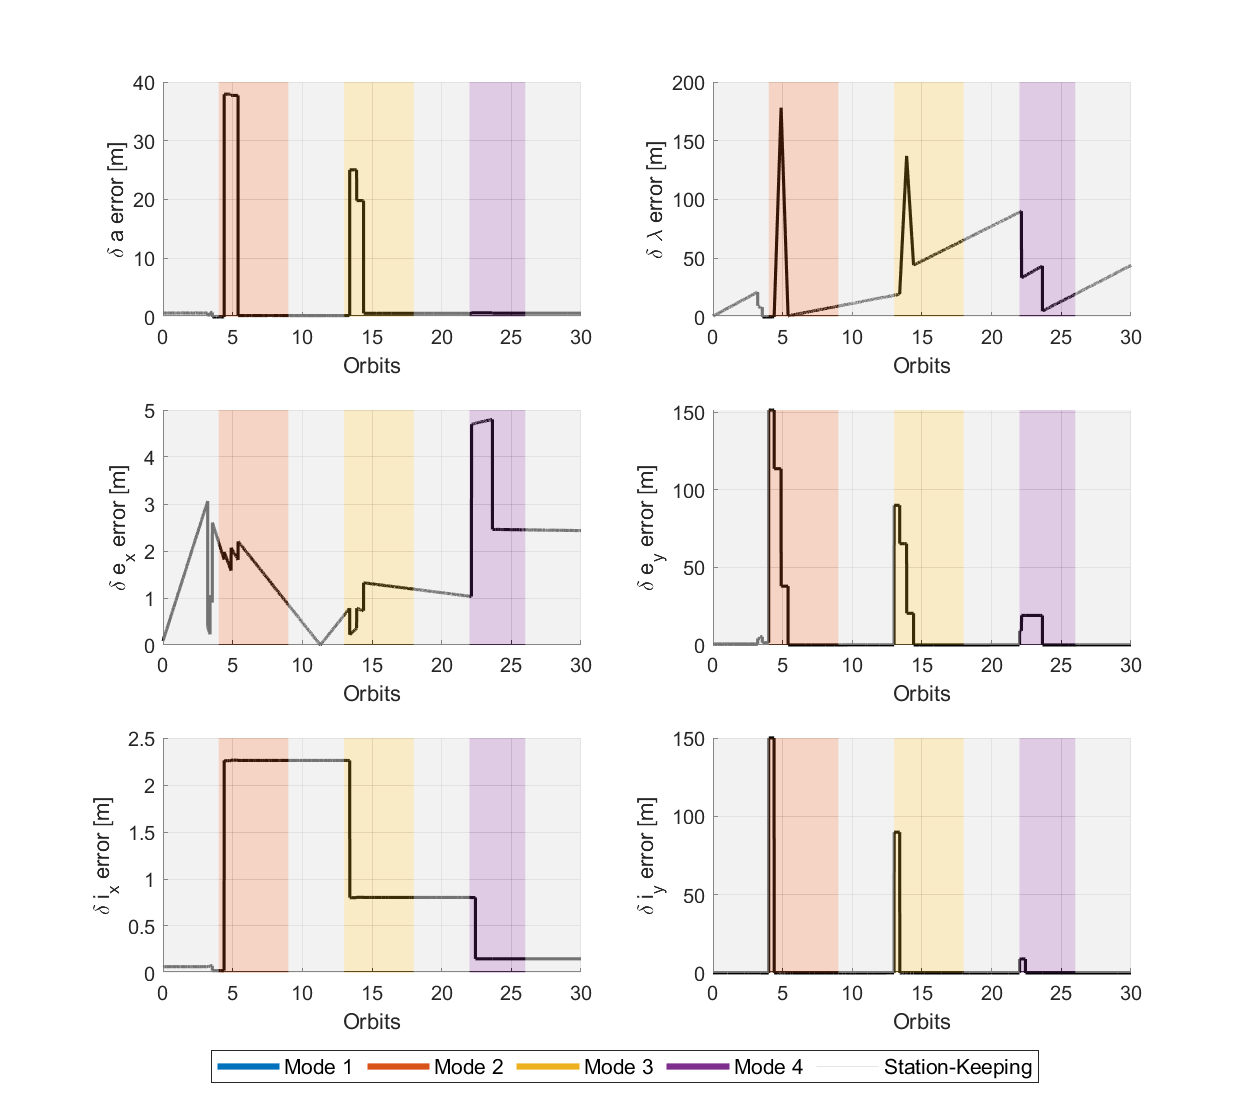
\includegraphics[width=0.75\linewidth]{sim/figures/PS5/ROE_error_over_time_modes_SV3.png}
    \caption{Tracking error between actual and desired ROE plotted for all modes in ROE time history}
    \label{fig:roe_error_time_modes}
\end{figure}

Figure \ref{fig:delta_v_modes} shows the delta-v magnitudes in the RTN directions throughout each control mode. As expected, delta-v magnitudes are on the order of mm/s. The magnitudes decrease in size as the desired change in ROE decreases throughout the modes. Additionally, the magnitudes in the normal direction are multiple times larger than those in radial or tangential. This arises from the fact that inclination maneuvers are much more expensive than eccentricity maneuvers. Since each mode changes relative eccentricity and relative inclination by the exact same magnitude, the inclination maneuver is going to have to be larger. 
\begin{figure}[H]
    \centering
    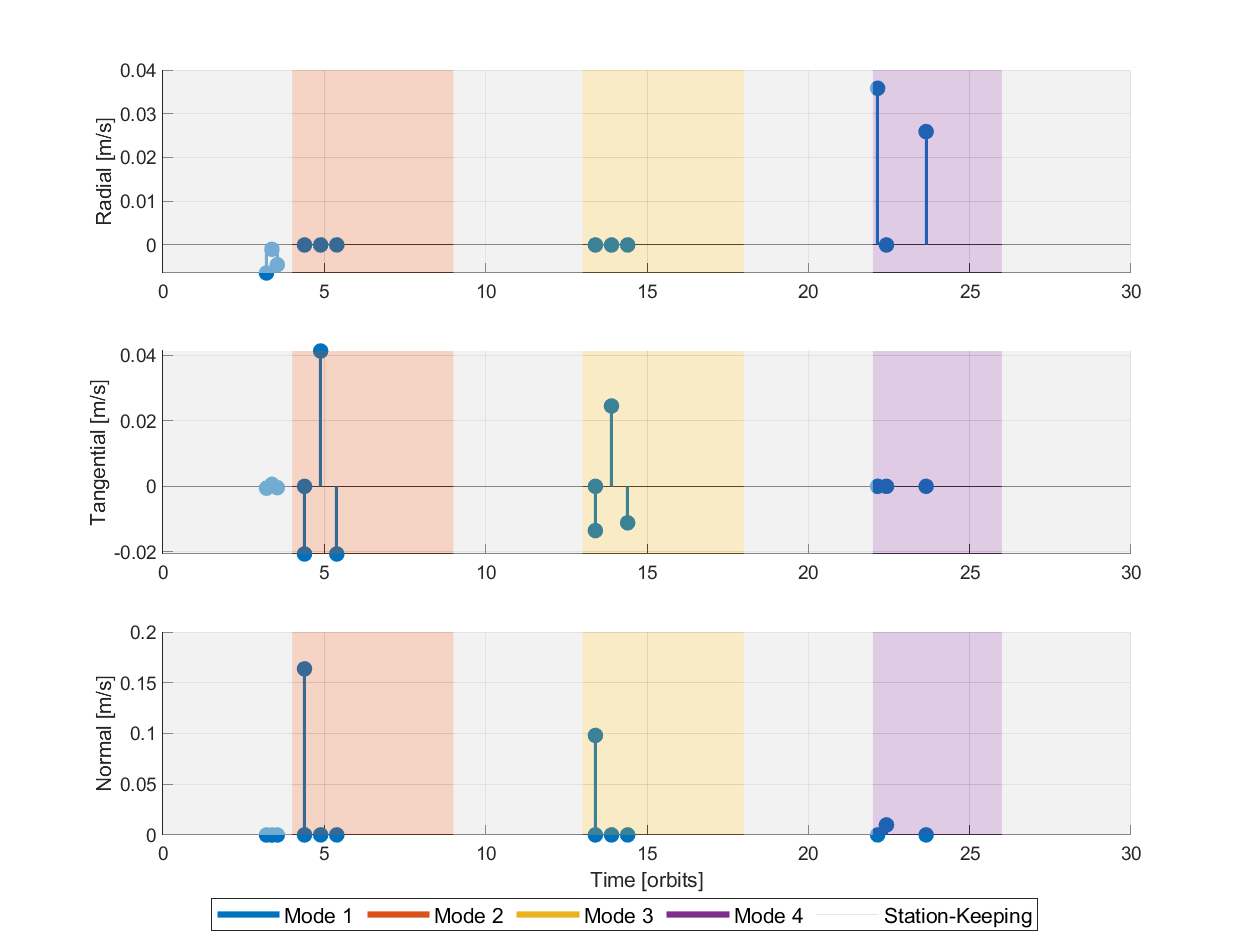
\includegraphics[width=0.75\linewidth]{sim/figures/PS5/delta_v_timeline_modes_SV3.png}
    \caption{Actual delta-v of control maneuvers over time}
    \label{fig:delta_v_modes}
\end{figure}

As a point of comparison, the theoretical delta-v lower bound can be calculated as follows:
\begin{align*}
\Delta v_{\text{ecc}} &= \frac{1}{2} \cdot n \cdot a \cdot \left\| \Delta \delta\vec{e} \right\| \\
\Delta v_{\text{inc}} &= n \cdot a \cdot \left\| \Delta \delta\vec{i} \right\| \\
\Delta v_{\text{lb}} &= \sqrt{\Delta v_{\text{ecc}}^2 + \Delta v_{\text{inc}}^2}
\end{align*}
Note that only changes in ROEs were in $\delta e$ and $\delta i$, which is why delta-v lower bound can be calculated as the norm of the along-track and cross-track delta-v's. 

Table \ref{tab:dv_comparison} compares the total delta-v with the theoretical lower-bound. 
% The actual delta-v's were approximately double the theoretical lower-bound for each mode. This suggests that there is room for improvement in optimizing the delta-v cost, which methods like reachable set theory could offer. 
The actual $\Delta v$ values were usually around 1.5x the lower bound values, which we deem as an acceptable inefficiency for the control of the $\delta \lambda$, $\delta a$, and $\delta e$. In Mode 4, the $\Delta v$ used is much higher than the lower bound because of the use of radial burns, as justified in Table \ref{tab:mode_control_methods}.
\begin{table}[h!]
\centering
\begin{tabular}{|c|c|c|}
\hline
\textbf{Mode} & \textbf{Total }$\Delta v$ \textbf{(m/s)} & \textbf{Lower Bound (m/s)} \\
\hline
2 & 0.2463 & 0.1830 \\
3 & 0.1472 & 0.1098 \\
4 & 0.07156 & 0.0110 \\
\hline
\end{tabular}
\caption{Total delta-$v$ compared with theoretical lower bounds for each maneuver mode}
\label{tab:dv_comparison}
\end{table}

% As mentioned previously, the station-keeping mode was treated separately to the other modes for the time being. The algorithm for station keeping is provided in Algorithm \ref{alg:station_keeping}. Ultimately, the station-keeping mode will be integrated into the full control system to prevent drift in ROEs when maintaining a formation. Figures \ref{fig:roe_planes_stk} and \ref{fig:roe_time_stk} show the current performance of the station-keeping control method. While there is still some erroneous behaviors, the control method successfully prevents drift in $\delta \lambda$ which is key for our formation to stay centered around the Target. The keep-in zone was set to a 1-meter radius circle centered on the desired ROEs. The control method is generally able to keep errors to below 5 meters. In future work, the unexpected behavior towards the end of the time series will be addressed. Also, the keep-in zone of 1 meter might be too tight for the current formulation, leading to this undesired behavior. 

% \begin{figure}[H]
%     \centering
%     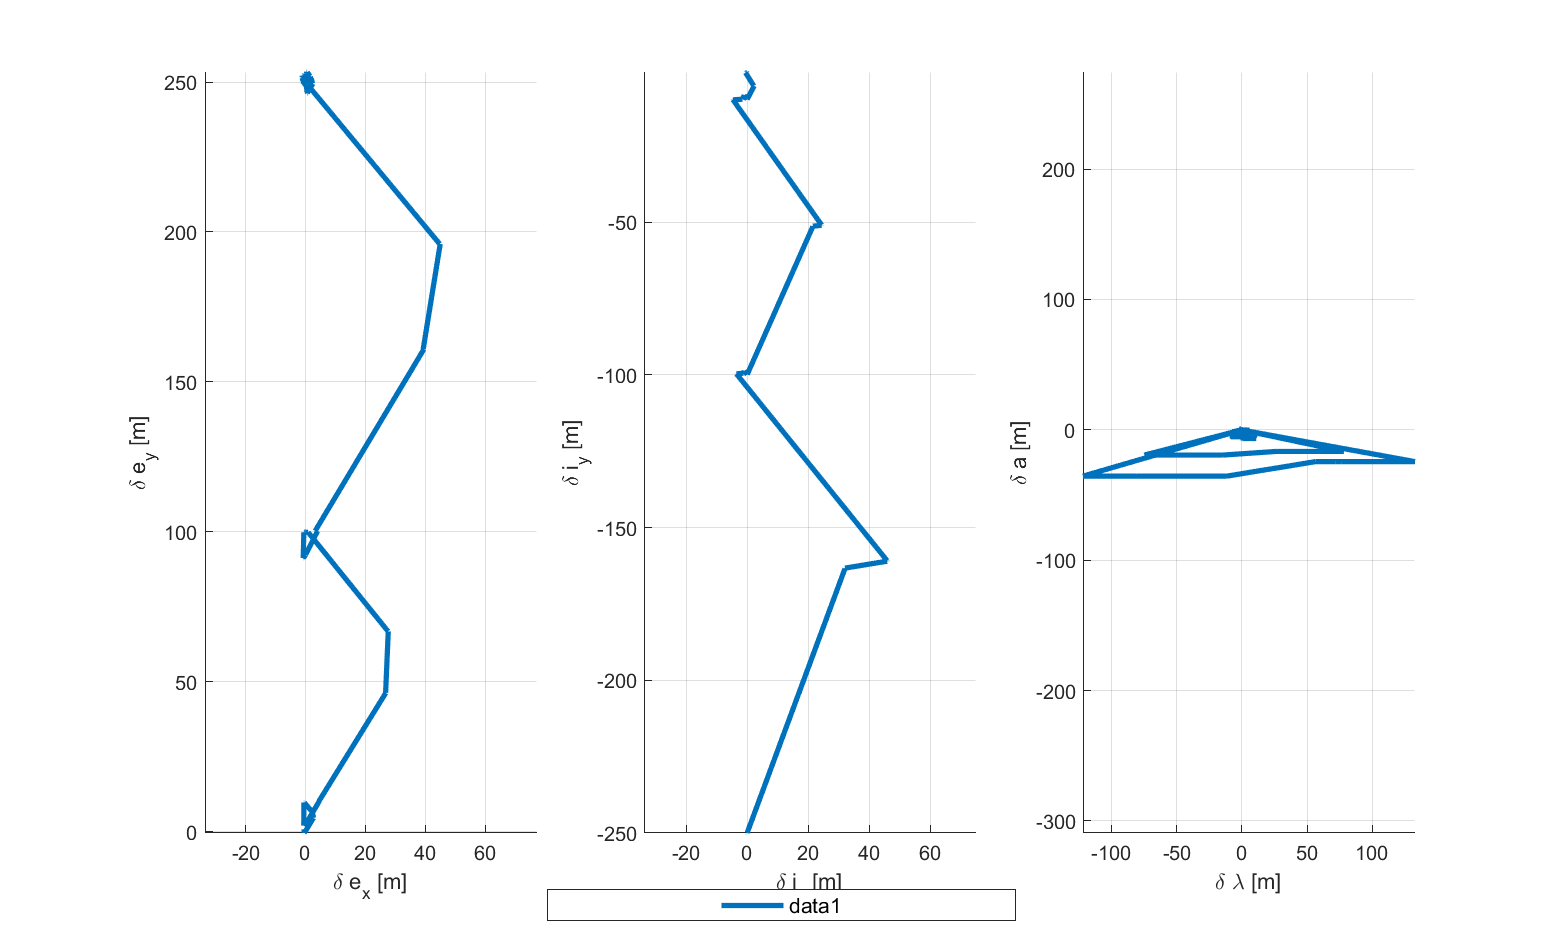
\includegraphics[width=0.7\linewidth]{sim/figures/PS5/ROE_planes_SV3.png}
%     \caption{Station-keeping mode in ROE planes}
%     \label{fig:roe_planes_stk}
% \end{figure}

% \begin{figure}[H]
%     \centering
%     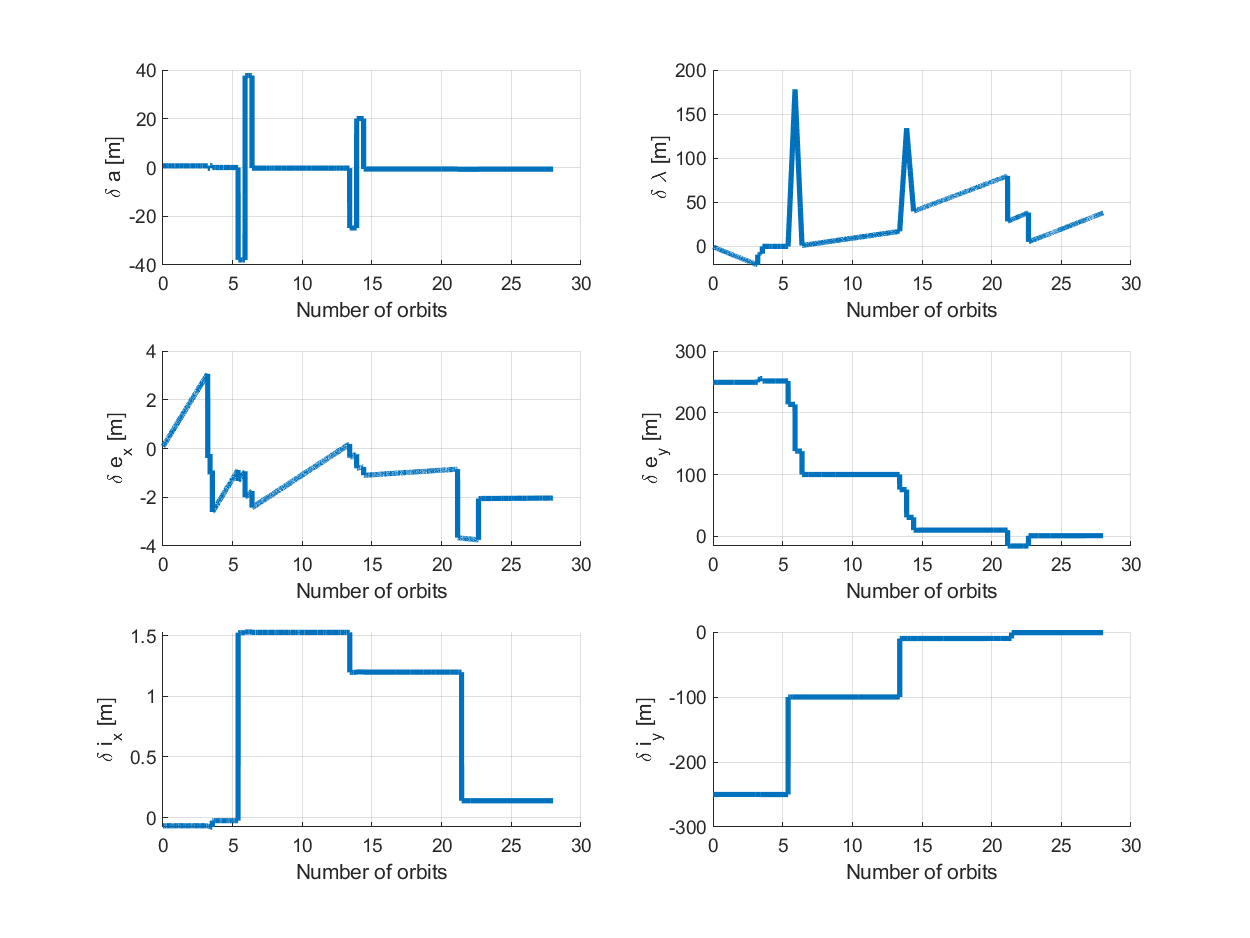
\includegraphics[width=0.7\linewidth]{sim/figures/PS5/ROE_over_time_SV3.png}
%     \caption{Station-keeping mode in ROE time history}
%     \label{fig:roe_time_stk}
% \end{figure}

